\input ../SlidePreamble
\input ../preamble

\begin{document}

{\Huge

  \centerline{\bf TTIC 31230, Fundamentals of Deep Learning}
  \bigskip
  \centerline{David McAllester, April 2019}


\vfill
\centerline{\bf AlphaZero}
\vfill
\vfill

\slide{AlphaGo Fan (October 2015)}

AlphaGo Defeats Fan Hui, European Go Champion.

\vfill
\centerline{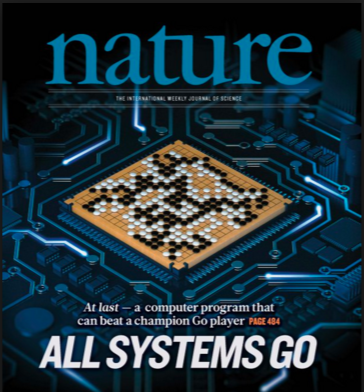
\includegraphics[width=4in]{../images/alphago}}

\slide{AlphaGo Lee (March 2016)}

\vfill
\centerline{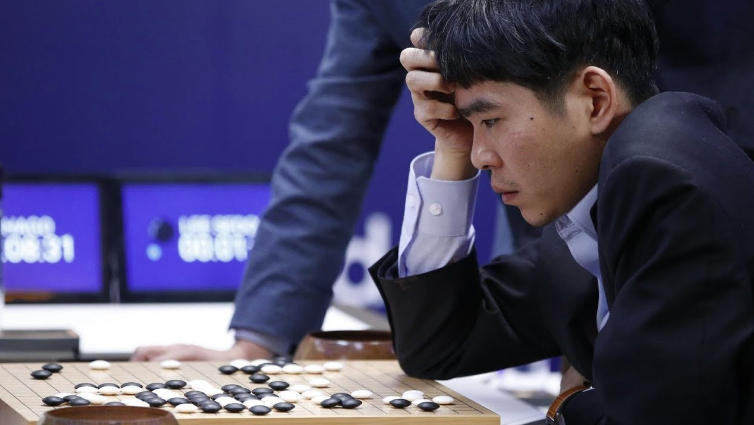
\includegraphics[width=8in]{../images/alphagolee}}

\slide{AlphaGo Zero vs. Alphago Lee (April 2017)}

{\bf AlphaGo Lee:}

\begin{itemize}
\item Trained on both human games and self play.
  
\item Trained for Months.

\item Run on many machines with 48 TPUs for Lee Sedol match.
\end{itemize}

{\bf AlphaGo Zero:}
\begin{itemize}
\item Trained on self play only.
  
\item Trained for 3 days.

\item Run on one machine with 4 TPUs.

\item Defeated AlphaGo Lee under match conditions 100 to 0.
\end{itemize}

\slide{AlphaZero Defeats Stockfish in Chess (December 2017)}

AlphaGo Zero was a fundamental algorithmic advance for general RL.

\vfill
The general RL algorithm of AlphaZero is essentially the same as that of AlphaGo Zero.

\slide{AlphaGo}

AlphaGo trains:

\begin{enumerate}
\item a fast rollout policy.

\item an imitation policy network.

\item a self-play policy network.

\item a value network trained to predict self-play rollout values.
\end{enumerate}

\vfill
No tree search is used in training --- in (3) and (4) ``self-play'' is just policy network rollouts.

\slide{1. Fast Rollout Policy}

Softmax of linear combination of (hand designed) pattern features.

\vfill
An accuracy of 24.2\%, using just 2 $\mu$s to select an action, rather than 3 ms for the policy network.

\slide{2. Imitation Policy Network}

\centerline{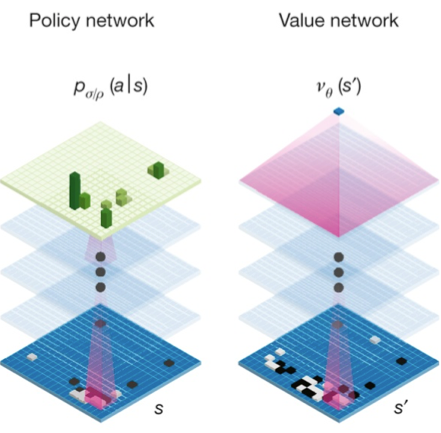
\includegraphics[height=3.0in]{../images/alphagoArchitecture2}}

\centerline{[Silver et al.]}

\vfill
Networks have 13 Layers of $5\times 5$ filters on 256 channels

\vfill
The immatation policy network is trained from from 30 million positions from the KGS Go Server.

\slide{3. Self-Play Policy Network}

Build a replay buffer by runing the self-play network against versions of itself to get (expensive) rollouts $a_1,b_1,a_2,b_2,\ldots,a_N,b_N$ with value $z$.

\vfill
``Self-play'' just draws moves from the policies --- there is no tree search in training.

\vfill
Draw rollouts from the replay buffer and update the network with REINFORCE.

$$\mathrm{for}\;t\;\;\;\;\;\;\;\Theta_\pi \;\pluseq\; \eta \;z\; \nabla_{\Theta_\pi} \;\ln \pi(a_t|s_t;\Theta_\pi)$$

\slide{4. Value Network}

Using self-play of the final self-play network policy we generate a database of 30 million pairs $(s,z)$ where $s$ is a board position and $z \in \{-1,1\}$ is an outcome
and each pair is from a different game.

\vfill
Again, ``self-play'' just selects moves from the policies --- there is no tree search in training.

\vfill
We then train the value network on the pairs $(s,z)$ in this database.

\vfill
$$\Theta^* = \argmin_\Theta \expectsub{(s,z)}{(V(s,\Theta) - z)^2}$$

\slide{Tournament Play uses Tree Search}

Rollout position evaluation (Bruegmann, 1993)

\vfill
Monte Carlo Tree Search (MCTS) (Bruegmann, 1993)

\vfill
Upper Confidence Bound (UCB) Bandit Algorithm (Lai and Robbins 1985)

\vfill
Upper Confidence Tree Search (UCT) (Kocsis and Szepesvari, 2006)

\slide{Rollouts and MCTS (1993)}

To estimate the value of a position (who is ahead and by how much)
run a cheap stochastic policy to generate a sequence of moves (a rollout) and see who wins.

\vfill
Do a selective tree search using rollout averages for position evaluation.

\slide{(One Armed) Bandit Problems}

Consider a set of choices (different slot machines).

Each choice gets a stochastic reward.

\vfill
We can select a choice and get a reward as often as we like.

\vfill
We would like to determine which choice is best and also to get reward as quickly as possible.

\slide{The Upper Confidence Bound (UCB) Algorithm}

For each choice (bandit) $a$ construct a confidence interval for its average reward.

\vfill
$$\mu = \hat{\mu} \pm 2\sigma/\sqrt{n}$$

\vfill
$$\mu(a) \leq \hat{\mu}(a) + U(N(a))$$

\vfill
Always select

$$\argmax_a \hat{\mu}(a) + U(N(a))$$

\slide{The Upper Confidence Tree (UCT) Algorithm}

The UCT algorithm grows a tree by running ``simulations''.

\vfill
Each simulation descends into the tree to a leaf node, expands that leaf, and returns a value.

\vfill
In the UTC algorithm each move choice at each position is treated as a bandit problem.

\vfill
We select the child (bandit) with the the lowest upper bound as computed from revious simulations selecting that child.

\slide{More Details}

When a leaf is expanded each new leaf is assigned a value, originally by averaging random rollouts.

\vfill
In AlphaGo each new leaf $s$ is assigned the value
$$\lambda V_\Phi(s) + (1-\lambda)V'(s)$$
where $V_\Phi(s)$ is the value of the value network and $V'(s)$ is the value of a fast rollout from $s$.

\vfill
Each new leaf is considered to have be ``visited'' once by a simulation which assigned it the above value.

\vfill
The simulation returns as a value to its parent nodes the largest value of the new leaves.

\slide{More Details}

At a non-leaf node an AlphaGo simulation selects the move

$$\argmax_a \;\hat{\mu}(s,a) + \lambda \pi_\Phi(a|s)\frac{\sqrt{N(s)}}{N(s,a)}$$

\vfill
$N(s,a) \geq 1$ is the number of sims that have visited $(s,a)$.

\vfill
$N(s)$ is the number of sims that have visited $s$.

\vfill
$\hat{\mu}(s,a)$ is the average value of the sims that have visited $(s,a)$.


\vfill
$\pi_\Phi(a|s)$ is the {\bf imitation learned} action probability.

\vfill
Eventually we select the root move $\argmax_a\;N(s,a)$.

\slide{AlphaGo Zero}

\begin{itemize}
\item There is no fast rollout policy or imitation policy --- just a self-play policy network and a self-play value network.

\vfill
\item No rollouts are ever used --- just self-play UCT with leaf values computed by the value network alone.

\vfill
\item The networks are replaced with Resnet.

\vfill
\item A single dual-head network is used for both policy and value.  
\end{itemize}

\slide{Learning from Tree Search}

UTC tree search is used to generate a complete self-play game.

Move selection during simulations is done using

$$\argmax_a \;\hat{\mu}(s,a) + \lambda \frac{\pi_\Phi(a|s)}{N(s,a)}$$

\vfill
Each self-play game has a final outcome $z$ and generates data $(s,\pi,z)$ for each position $s$ in the game where
$$\pi(a) \propto N(s,a)^\beta$$
where $\beta$ is a temperature hyperparameter and $z$ is the final value of the game.

\vfill
This data is collected in a replay buffer.

\slide{Learning from Tree Search}

\vfill
Learning is done from this replay buffer using the following objective on a single dual-head network.

\vfill
$$\Phi^*\; = \;\argmin_\Phi \;E_{(s,\pi,z) \sim \mathrm{Replay},\;a \sim \pi}\;\left(\begin{array}{l} (V_\Phi(s) - z)^2 \\ \\ - \lambda_1\log \pi_\Phi(a|s) \\ \\ + \lambda_2||\Phi||^2\end{array}\right)$$

\slide{Selecting Root Moves}

During self-play we have two forms of move selection.

\begin{itemize}
\item Selecting a child during a simulation as part of tree-growth.
\item Selecting a root move to make progress in the actual play of the game.
\end{itemize}

\vfill
In AlphaGo root moves were selected by $\argmax_a N(s,a)$.

\vfill
In AlphaZero self-play, exploration is maintained by selecting root moves in proportion to $N(s,a)$ for the first 30 moves and then
selecting $\argmax_a\;N(s,a)$ beyond 30 moves.

\vfill
Throughout the game a random root move is used with probability $\epsilon << 1$.

\slide{Training Time}

4.9 million games of self-play

\vfill
0.4s thinking time per move

\vfill
About 8 years of thinking time in training.

\vfill
Training took just under 3 days --- about 1000 fold parallelism.

\slide{Elo Learning Curve}

\centerline{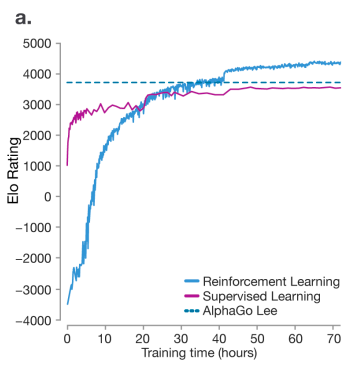
\includegraphics[height = 5in]{../images/alphalearning1}}

\slide{Learning Curve for Predicting Human Moves}

\centerline{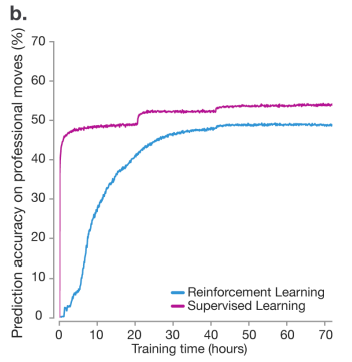
\includegraphics[height = 5in]{../images/alphalearning2}}

\slide{Ablation Study for Resnet and Dual-Head}

\centerline{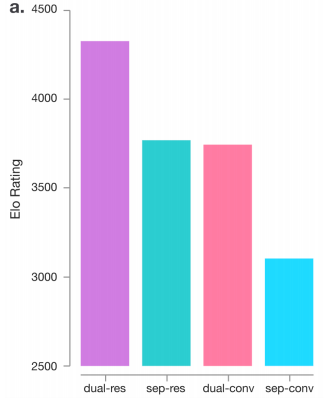
\includegraphics[height = 5in]{../images/alphaablation}}


\slide{Increasing Blocks and Training}

Increasing the number of Resnet blocks form 20 to 40.

\vfill
Increasing the number of training days from 3 to 40.

\vfill
Gives an Elo rating over 5000.

\slide{Final Elo Ratings}

\centerline{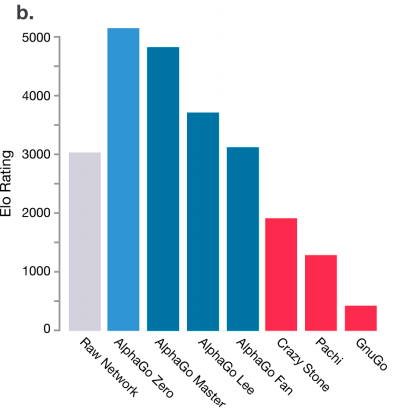
\includegraphics[height = 5in]{../images/alpha40}}

\slide{AlphaZero --- Chess and Shogi}

Essentially the same algorithm with the input image and output images modified to represent to game position and move options respective.

\vfill
Minimal representations are used --- no hand coded features.

\vfill
Three days of training.

\vfill
Tournaments played on a single machine with 4 TPUs.

\slide{Alpha vs. Stockfish}

From white Alpha won 25/50 and lost none.

\vfill
From black Alpha won 3/50 and lost none.

\vfill
Alpha evaluates 70 thousand positions per second.

\vfill
Stockfish evaluates 80 million positions per second.

\slide{Checkers is a Draw}

In 2007 Jonathan Schaeffer at the University of Alberta showed that checkers is a draw.

\vfill
Using alpha-beta and end-game dynamic programming, Schaeffer computed drawing strategies for each player.

\vfill
This was listed by Science Magazine as one of the top 10 breakthroughs of 2007.

\vfill
Is chess also a draw?

\slide{Grand Unification}

AlphaZero unifies chess and go algorithms.

\vfill
This unification of intuition (go) and calculation (chess) is surprising.

\vfill
This unification grew out of go algorithms.

\vfill
But are the algorithmic insights of chess algorithms really irrelevant?

\slide{Chess Background}

The first min-max computer chess program was described by Claude Shannon in 1950.

\vfill
Alpha-beta pruning was invented by various people independently, including John McCarthy, about 1956-1960.

\vfill
Alpha-beta has been the cornerstone of all chess algorithms until AlphaZero.


\slide{Alpha-Beta Pruning}

\begin{verbatim}
def MaxValue(s,alpha,beta):
   value = alpha
   for s2 in s.children():
     value = max(value, MinValue(s2,value,beta))
     if value >= beta: break()
   return value

def MinValue(s,alpha,beta):
   value = beta
   for s2 in s.children():
     value = min(value, MaxValue(s2,alpha,value))
     if value <= alpha: break()
   return value
\end{verbatim}

\slideplain{Conspiracy Numbers}

Conspiracy Numbers for Min-Max search, McAllester, 1988

\vfill
Each node $s$ has a min-max value $V(s)$ determined by the leaf values.

\vfill
For any positive integer $N$ and potential value $V$ we define $L(N,V)$ to be the set of leaf nodes $s_1$ such that
there exist $N-1$ other leaf nodes $s_2$, $\ldots$, $s_N$ such that by changing the values of $s_1$, $\ldots$, $s_N$ the root node
can be changed to $V$.


\vfill
{\bf Algorithm:}


\vfill
Repeatedly select some $N$ and $V$ such that $L(N,V)$ is non empty and expand some leaf in $L(N,V)$.

\ignore{
\slide{Simulation}

To find an upper-confidence leaf for the root and value $U$:

\vfill
At a max node pick the child minimizing $N(s,U)$.

\vfill
At a min node select any child $s$ with $V(s) < U$.

\vfill
\slide{Refinement}

Let the static evaluator associate leaf nodes with values $U(s,N)$ and $L(s,N)$
}

\slide{END}

}
\end{document}


